% `template.tex', a bare-bones example employing the AIAA class.
%
% For a more advanced example that makes use of several third-party
% LaTeX packages, see `advanced_example.tex', but please read the
% Known Problems section of the users manual first.
%
% Typical processing for PostScript (PS) output:
%
%  latex template
%  latex template   (repeat as needed to resolve references)
%
%  xdvi template    (onscreen draft display)
%  dvips template   (postscript)
%  gv template.ps   (onscreen display)
%  lpr template.ps  (hardcopy)
%
% With the above, only Encapsulated PostScript (EPS) images can be used.
%
% Typical processing for Portable Document Format (PDF) output:
%
%  pdflatex template
%  pdflatex template      (repeat as needed to resolve references)
%
%  acroread template.pdf  (onscreen display)
%
% If you have EPS figures, you will need to use the epstopdf script
% to convert them to PDF because PDF is a limmited subset of EPS.
% pdflatex accepts a variety of other image formats such as JPG, TIF,
% PNG, and so forth -- check the documentation for your version.
%
% If you do *not* specify suffixes when using the graphicx package's
% \includegraphics command, latex and pdflatex will automatically select
% the appropriate figure format from those available.  This allows you
% to produce PS and PDF output from the same LaTeX source file.
%
% To generate a large format (e.g., 11"x17") PostScript copy for editing
% purposes, use
%
%  dvips -x 1467 -O -0.65in,0.85in -t tabloid template
%
% For further details and support, read the Users Manual, aiaa.pdf.


% Try to reduce the number of latex support calls from people who
% don't read the included documentation.
%


\typeout{}\typeout{If latex fails to find aiaa-tc, read the README file!}
%


\documentclass[]{aiaa-tc}% insert '[draft]' option to show overfull boxes
\usepackage{float}
\usepackage{epstopdf}
\usepackage{amsmath}

\title{Single-Axis Control of a Solar Sail Through a Gimbal}

\author{
	Johnathan Clouse%
	\thanks{Graduate Students, Aerospace Engineering Sciences, 1111 Engineering Drive, Boulder, CO, 80309-0429}\\
	{\normalsize\itshape
		University of Colorado, Boulder, CO, 80309-0429, USA}
}

% Define commands to assure consistent treatment throughout document
\newcommand{\eqnref}[1]{(\ref{#1})}
\newcommand{\class}[1]{\texttt{#1}}
\newcommand{\package}[1]{\texttt{#1}}
\newcommand{\file}[1]{\texttt{#1}}
\newcommand{\BibTeX}{\textsc{Bib}\TeX}

\usepackage[euler]{textgreek}
\usepackage[colorlinks=true]{hyperref}
\hypersetup{urlcolor=cyan}

\usepackage{listings}
\usepackage{color} %red, green, blue, yellow, cyan, magenta, black, white
\definecolor{mygreen}{RGB}{28,172,0} % color values Red, Green, Blue
\definecolor{mylilas}{RGB}{170,55,241}

\usepackage{tablefootnote}
\usepackage{graphicx}
\usepackage{amsmath}
\usepackage{bm}
\usepackage{subfigure}
%\usepackage{subcaption}

\definecolor{mylilas}{RGB}{170,55,241}

% See p.105 of "TeX Unbound" for suggested values.
% See pp. 199-200 of Lamport's "LaTeX" book for details.
%   General parameters, for ALL pages:
\renewcommand{\topfraction}{0.9}	% max fraction of floats at top
\renewcommand{\bottomfraction}{0.8}	% max fraction of floats at bottom
%   Parameters for TEXT pages (not float pages):
\setcounter{topnumber}{2}
\setcounter{bottomnumber}{2}
\setcounter{totalnumber}{4}     % 2 may work better
\setcounter{dbltopnumber}{2}    % for 2-column pages
\renewcommand{\dbltopfraction}{0.9}	% fit big float above 2-col. text
\renewcommand{\textfraction}{0.07}	% allow minimal text w. figs
%   Parameters for FLOAT pages (not text pages):
\renewcommand{\floatpagefraction}{0.7}	% require fuller float pages
% N.B.: floatpagefraction MUST be less than topfraction !!
\renewcommand{\dblfloatpagefraction}{0.7}	% require
    \makeatletter
    \renewcommand\l@section{\@dottedtocline{2}{1.5em}{3em}}
    \makeatother
    
\begin{document}
	

	
	\maketitle
	
	\begin{abstract}
		\noindent 
		
	\end{abstract}
	
	\newpage
	
	\tableofcontents
	
	\newpage

	\section{Introduction}
Single-axis control of a solar-sail-driven interplanetary spacecraft (sailcraft) is proposed.  The attitude control system will be responsible for ensuring that the steering angle between the force and velocity vectors is within the tolerance necessary for an interplanetary voyage.  This steering angle is dependent on the mission parameters and the orbital position of the spacecraft. It, and the sun vector, will be treated as external commands to the system. The spacecraft will perform all its thrusting in the orbit plane.
	
	\vspace{5 mm}
	
The primary actuation mechanism will be a gimbaled control boom between the sail subsystem and the spacecraft bus, which contains the majority of the spacecraft mass.  With the center of mass between the thrust point and the sun, expected disturbances will cause oscillation about some angle between the sun and the axis normal to the sail, $\alpha$, for a locked gimbal.  Changing the gimbal angle, $\delta$, will dampen this oscilation with the right conrol law. Roll and pitch angles wil be held to zero for this analysis. Star trackers will determin attitude.
	
	\vspace{5 mm}

The state-space model is expected to have four states: the sun angle ($\alpha$), the rate of the sun angle ($\dot{\alpha}$), the gimbal angle ($\delta$), and the gimbal angle rate ($\dot{\delta}$).  Depending on the vane implementation, there may be up to two more states for vane angles.
	
	\vspace{5 mm}

The sail and boom will be modeled as rigid bodies, justified by the slow actuation of the gimbal throughout the flight. The sail will be modeled as a thin plate, rather than a billowed sail. Solar pressure torques (about the non-steered axis) will be controlled against. Disturbance torques from thruster firings may also be modeled. 
	
	\vspace{5 mm}

The state-space model will be obtained in a similar manner to that presented by Wie. The equations of motion for a gimbaled thrust vector are obtained for the yaw axis. 
	
	\vspace{5 mm}

System performance will be judged by the response to errors, both with a step-error and a flight-like error where the steering angle constantly-but-slowly changes. Mitigation of disturbance torques will also be examined.

	\section{State Space Representation}

	The equations of motion were linearized about the state $\alpha = \dot{\alpha} = \delta = \dot{\delta} =0$. This state is in equilibrium, due to the the force resulting from the solar radiation pressure acting through the sailcraft's center of mass.  Any disturbance to $\alpha$ would cause oscillation about $\alpha=0$. The linearized equations are shown below:

	\begin{equation}
\begin{bmatrix}
\dot{\alpha }\\ 
\ddot{\alpha}\\ 
\dot{\delta }\\ 
\ddot{\delta }
\end{bmatrix}=\begin{bmatrix}
0 & 1 & 0 & 0\\ 
0 & 0 & \frac{d}{J_s}F_n & 0\\ 
0 & 0 & 0 & 1\\ 
\frac{-m_pl}{m(J_p+\frac{m_sm_p}{m}l^2)}F_t & 0 & \frac{-m_pl}{m(J_p+\frac{m_sm_p}{m}l^2)}F_n & 0
\end{bmatrix}
\begin{bmatrix}
\alpha\\ 
\dot{\alpha}\\ 
\delta\\ 
\dot{\delta }
\end{bmatrix}
+
\begin{bmatrix}
0\\ 
-\frac{1}{J_s}\\ 
0\\ 
\frac{1}{J_p+\frac{m_sm_p}{m}l^{2}}
\end{bmatrix}T_{gimbal}
	\end{equation}
	\begin{equation}
y = \begin{bmatrix}
1 & 0 & 0 & 0
\end{bmatrix}x+\begin{bmatrix}
0
\end{bmatrix}u
	\end{equation}
	\begin{equation}
F_n=PA(1+\rho_s+\frac{2}{3}\rho_d)
	\end{equation}
	\begin{equation}
F_t=PA(1-\rho_s)
	\end{equation}
	
	\begin{table}[H]% no placement specified: defaults to here, top, bottom, page
		\begin{center}
			\caption{Sailcraft characteristics.}
			\label{t:Primary_variables}
			\begin{tabular}{|c|c|}
\hline 
Characteristic & Value  \\ \hline
$m_s$         &     40 kg\\
$m_p$         &      116 kg \\
$m$         &     156 kg \\
$J_s$   &     6000 kg$\cdot$m\textsuperscript{2} \\
$J_p$   &     20 kg$\cdot$m\textsuperscript{2} \\
$P$   &      4.563e-6 kg/m\textsuperscript{2}\\
$A_{sail}$       &     1800 m\textsuperscript{2} \\
$l$       &   2 m \\
$d$       &     1.487 m \\
$\rho_s$ &     0.8272 \\
$\rho_d$ &     -0.5949 \\
\hline
			\end{tabular}
		\end{center}
	\end{table}  

	Using the sailcraft characteristics in Table \ref{t:Primary_variables}, the eigenvalues are found to be:
	
	\vspace{5 mm}
{\centering
 $\lambda_i = \{\pm1.1200\times10^{-2}i, \pm5.9395\times10^{-4}i\}$.\par
}
	
	\vspace{5 mm}

	The complex eigenvalues with no real parts indicate that the uncontrolled, linearized system is marginally stable. It will oscillate undamped when perturbed by a small amount, but a large disturbance could excite the modes and make the output $y$ unbounded. However, as $\alpha$ and $\delta$ each approach $\pm$90$^{\circ}$, the assumption becomes invalid. Indeed, in Figure \ref{fig:Force_linearity}, one can see that a five-percent error between the non-linear and linearized sail force occurs at approximately $\pm$20$^{\circ}$.

	\vspace{5 mm}
	
	\begin{figure}[H]
		\centering
		\subfigure[Transverse force]{
			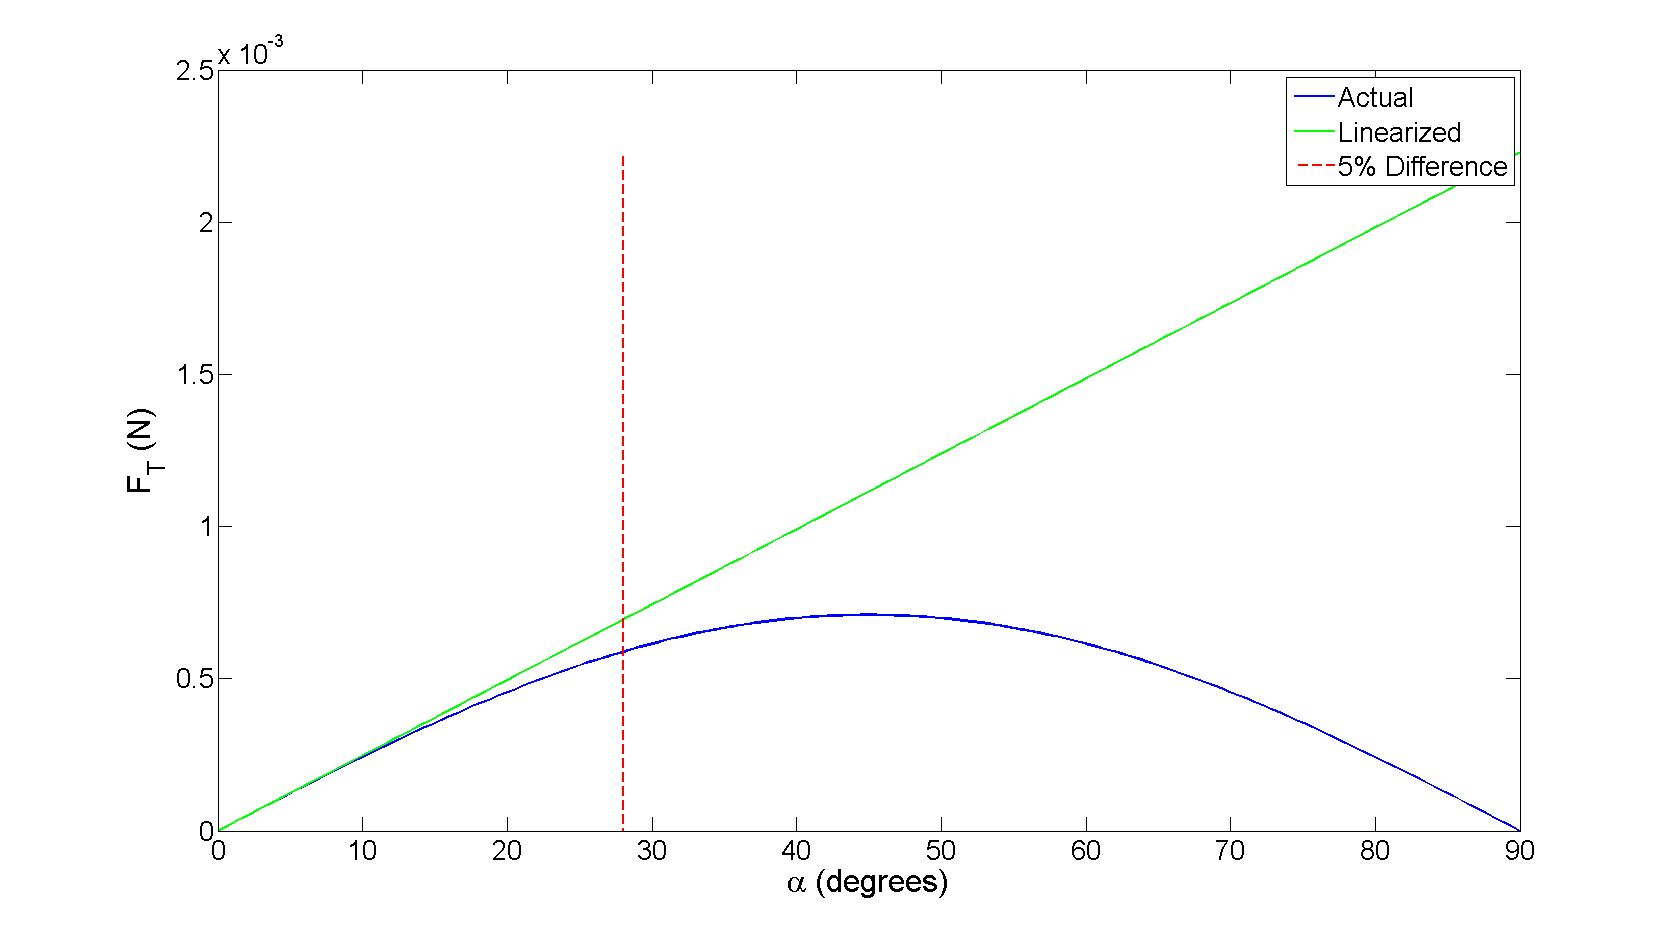
\includegraphics[width = 7.5cm]{FT_Soln.png}
		}
		\subfigure[Normal force]{
			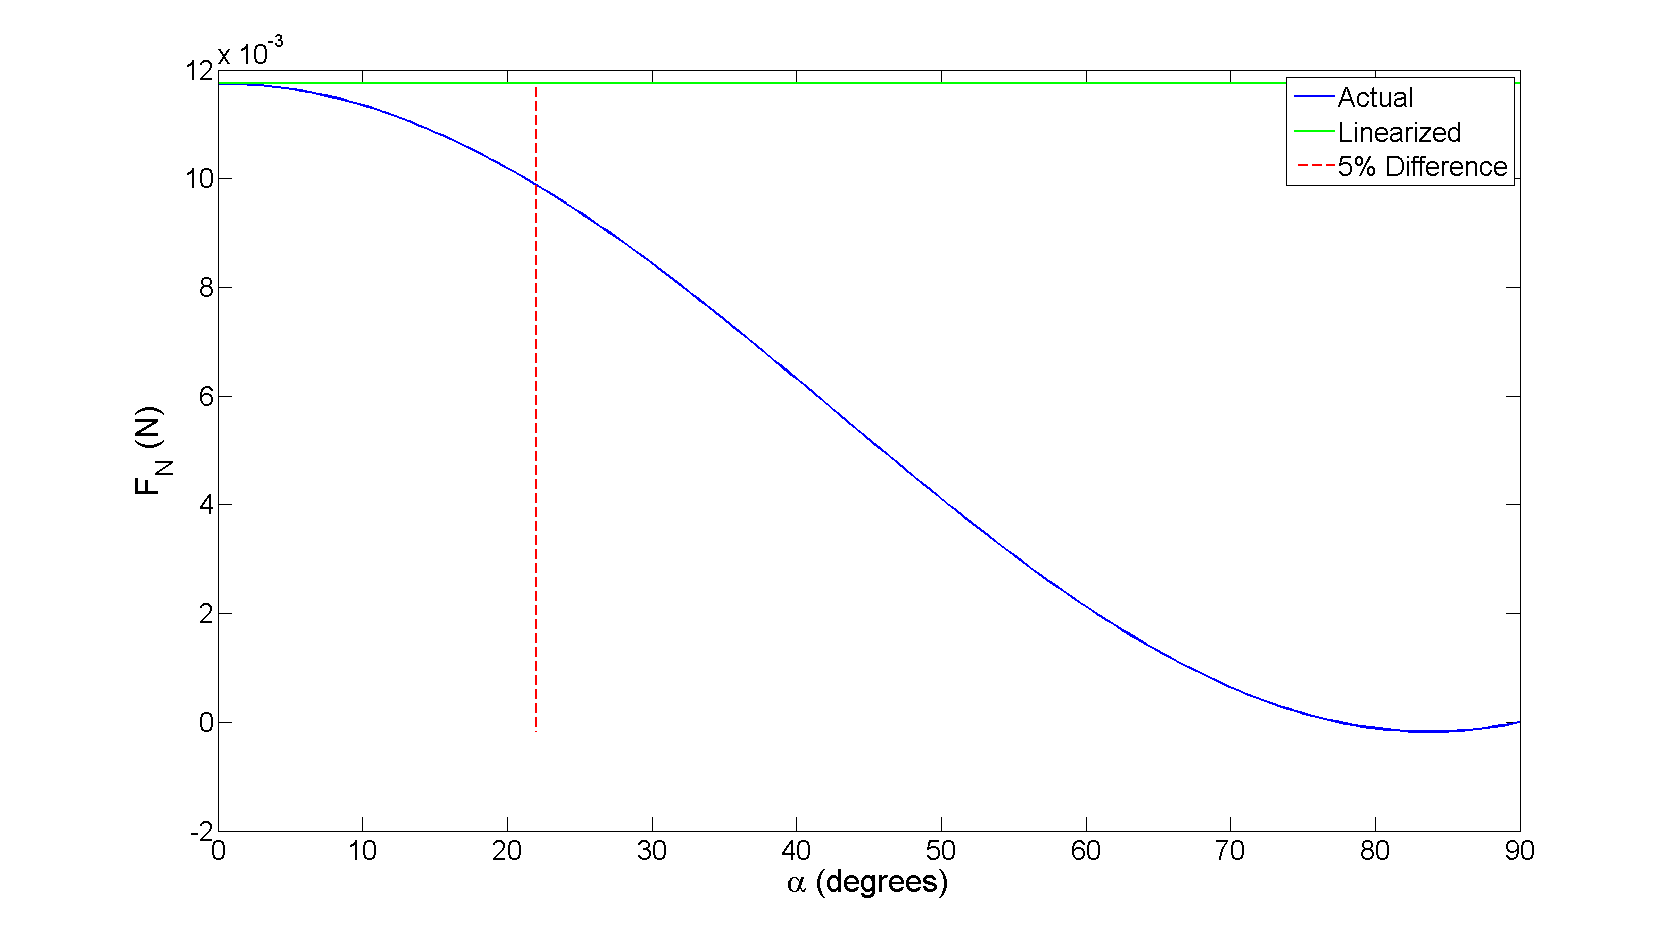
\includegraphics[width = 7.5cm]{FN_Soln.png}
		}
		\caption{Linear solutions of the sail forces vs. sun angle. }
		\label{fig:Force_linearity}
	\end{figure}	

	\vspace{5 mm}

	The controller will be constrained to keep the sun angle less than or equal to 20$^{\circ}$ to keep the system model within the realm of linearity. It will have to dampen the oscillations induced induced by disturbances so that the sail can provide a force in the desired direction. 

	\vspace{5 mm}
	\section{Homework 7}

	The system is found to be controllable since the four-row controllability matrix is full rank.

	\vspace{5 mm}

	For full-state feedback control, pole placement will have to be performed such that the real parts are negative. The gimbal angle cannot exceed $\pm$90$^{\circ}$, which is a physical constraint. To maintain the linearity-about-zero assumption, the sun angle $\alpha$ should not exceed $\pm$20$^{\circ}$. The controller will track the specified sun angle with zero steady-state error.  Due to the slow nature of the changing reference, a nearly-critical damped response will be sufficient.

	\vspace{5 mm}

	The system is found to be observable since the observability matrix is full rank.

	\vspace{5 mm}

	The uncontrolled step response of the system is shown in Figure \ref{fig:StepResp}. The response matches the eigenvalues: two sine waves superimposed on eachother, each corresponding to one of the complex conjugate pairs. Because the eigenvalues have no real part, the motion is undamped.

	\vspace{5 mm}

	\begin{figure}[H]
		\centering
			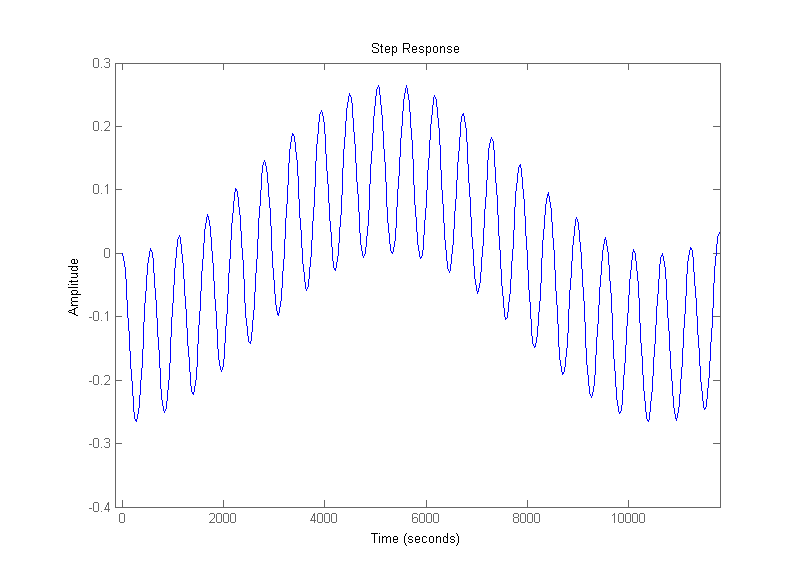
\includegraphics[width = 10cm]{StepResponse.png}
		\caption{Linear solutions of the sail forces vs. sun angle. }
		\label{fig:StepResp}
	\end{figure}	

	Reachability is determined by comparing the rank of the controllability matrix with the rank of the open-loop system. The controllability matrix $P$ turns out to be 

	\begin{equation}
P=\begin{bmatrix}
B & AB & A^2B &A^3B 
\end{bmatrix}=\begin{bmatrix}
            0 &     -1.6564\times10^{-4} &             0 &    4.6394\times10^{-9}\\ 
  -1.6564\times10^{-4} &               0 &    4.6394\times10^{-9} &             0\\ 
            0 &      7.4412\times10^{-3} &             0 &   -9.3875\times10^{-7}\\ 
   7.4412\times10^{-3} &               0 &   -9.3875\times10^{-7} &             0
\end{bmatrix}
	\end{equation}

The rank of the controllability matrix is 4, as is the rank of the system matrix $A$. Thus, the system is controllable. Because A is full rank, controllability implies reachability, so the system is actually reachable.

	\vspace{5 mm}

	Observability is determined by comparing the rank of the observability matrix with the rank of the open-loop system. The observability matrix $O$ is
	\begin{equation}
O=\begin{bmatrix}
C\\ 
CA\\ 
CA^2\\ 
CA^3
\end{bmatrix}=\begin{bmatrix}
    1.0000 &             0 &            0 &           0\\ 
             0 &    1.0000 &            0 &           0\\ 
   -1.2654\times10^{-8} &             0 &   6.2320\times10^{-7} &           0\\ 
             0 &   -1.2654\times10^{-8} &            0 &  6.2320\times10^{-7}
\end{bmatrix}
	\end{equation}

The rank of the observability matrix is 4. Thus, the system is observable.

	\section{State Feedback from Manual Pole Placement}
	The design parameters were chosen to be as follows: for a state at the origin, control the sun angle to 35$^{\circ}$ in 90 minutes (within 5\%) with no more than 10\% overshoot and without violating the actuator limits defined previously. This slew is actually fairly fast compared to the nominal steering, but would be useful for attitude maneuvers needed to meet payload or communications constraints, recovering from a fault en route. An integral term was also implemented to drive the steady-state error of the sun angle to zero while being robust to disturbances and plant errors. The poles were then chosen such that the dominant poles for a damped harmonic oscilator would have these characteristics. The other complex conjugate poles were placed to the left of the dominant poles by 0.1 on the real axis. The final pole was picked to be far to the left of the dominant poles, at -100. With the poles placed, the full-state feedback gains were:

\begin{equation}
\begin{aligned}
K &= \begin{bmatrix}
K_{\alpha} & K_{\delta} & K_{\dot{\alpha}} & K_{\dot{\delta}} & K_i
\end{bmatrix}\\ 
 &= \begin{bmatrix}
-3.7246\times10^5 & -5.9012\times10^7 & -5.4575\times10^3 & -1.3001\times10^6 & 1.2580\times10^3
\end{bmatrix}
\end{aligned}
\end{equation}

	Figure  \ref{fig:Controller1} shows the response of a sail starting at $\alpha=\delta=0^{\circ}$ being controlled to $\alpha = 35^{\circ}$.

	\vspace{5 mm}
	
	\begin{figure}[H]
		\centering
		\subfigure[$\alpha$ response]{
			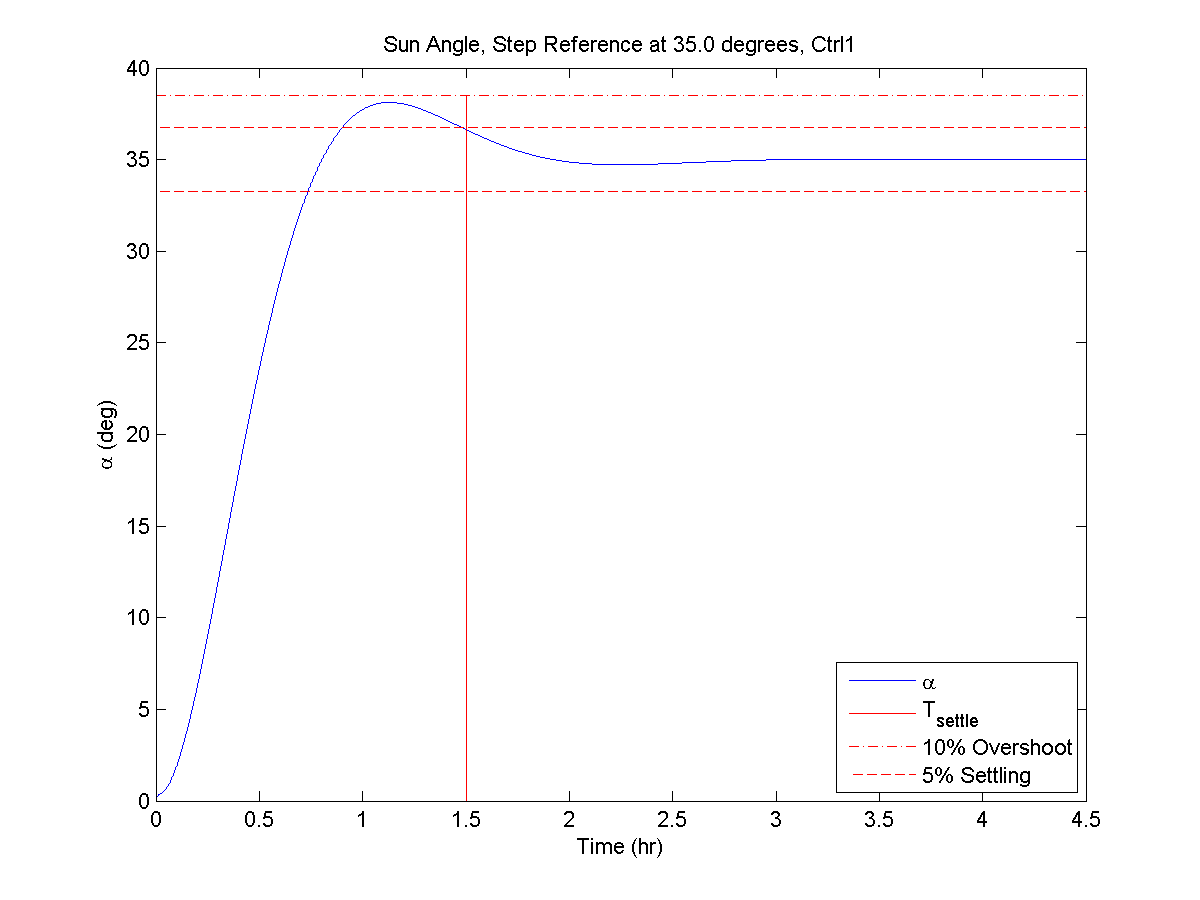
\includegraphics[width = 7.75cm]{Ctrl1_Alpha.png}
		}
		\subfigure[$\delta$ response]{
			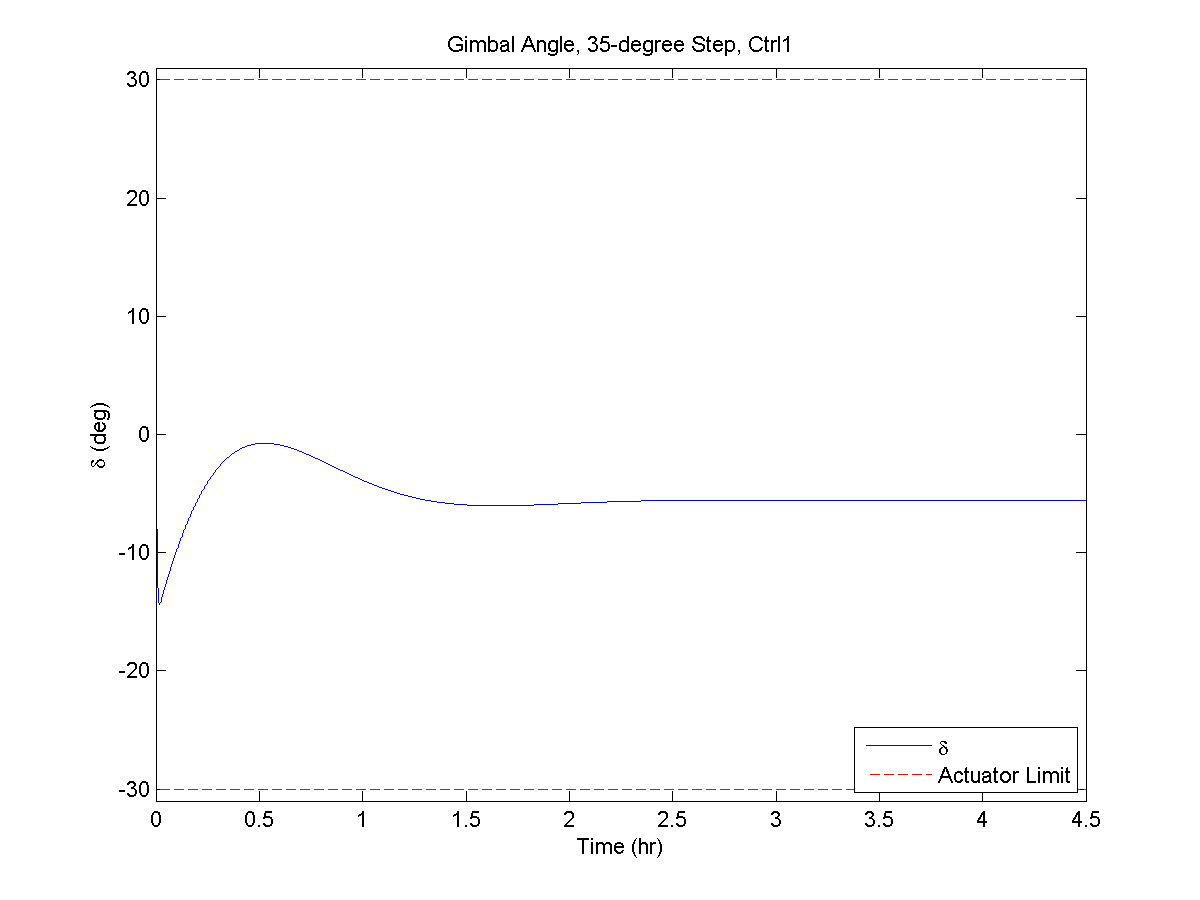
\includegraphics[width = 7.75cm]{Ctrl1_Delta.png}
		}
		\subfigure[Gimbal torque]{
			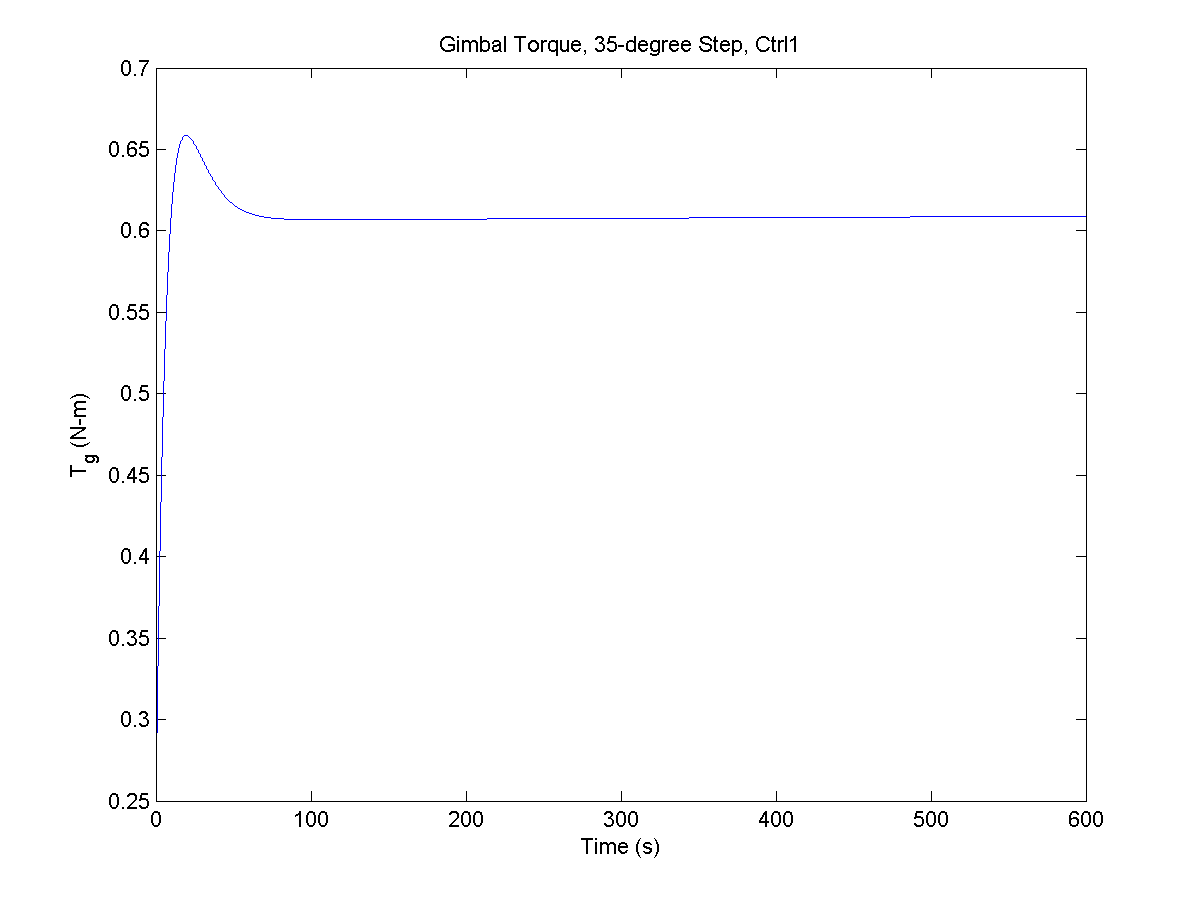
\includegraphics[width = 7.75cm]{Ctrl1_Torque.png}
		}
		\caption{System response of controller with manually placed poles, commanded $\alpha=35^{\circ}$. }
		\label{fig:Controller1}
	\end{figure}	

	One can see from the results that the controller met the design criteria. The underdamped motion of $\alpha$ is expected due to the complex-conjugate eigenvalue pairs. The gimbal tourque is a maximum of 0.35 N-m to maximize the initial change in $\alpha$, and settles the value required to hold the sail/bus configuration as $\alpha$ settles. The gimbal angle $\delta$ settles to a non-zero trim position to keep $\alpha$ at its reference value. This result is practical given that the actuator limit is not violated. The gimbal torque, which is the control effort, is also less compared to that of comparable systems [Wie].

	\section{Observer Design}

	A Luenberger observer was designed to reconstruct the state from sun-angle measurements. The Luenberger gains $L$ were tuned by placing poles on the negative-real axis until the previously-studied step response produced a gimbal angle within the limits and the gimbal torque was minimized for an observer error at the maximum sensor inaccuracy.

\begin{equation}
\begin{aligned}
L &= \begin{bmatrix}
L_{\alpha} & L_{\delta} & L_{\dot{\alpha}} & L_{\dot{\delta}} 
\end{bmatrix}\\ 
 &= \begin{bmatrix}
-3.7246\times10^5 & -5.9012\times10^7 & -5.4575\times10^3 & -1.3001\times10^6 
\end{bmatrix}
\end{aligned}
\end{equation}

	For an initial error of zero, the observer implementation performed the same as the previously-analyzed controlled system. However, with an error in sun angle of 0.05$^{\circ}$, the results differed. The previously-defined controller response with the observer implementation and initial error are shown in Figure  \ref{fig:Controller1Obs}.

	\begin{figure}[H]
		\centering
		\subfigure[$\alpha$ response]{
			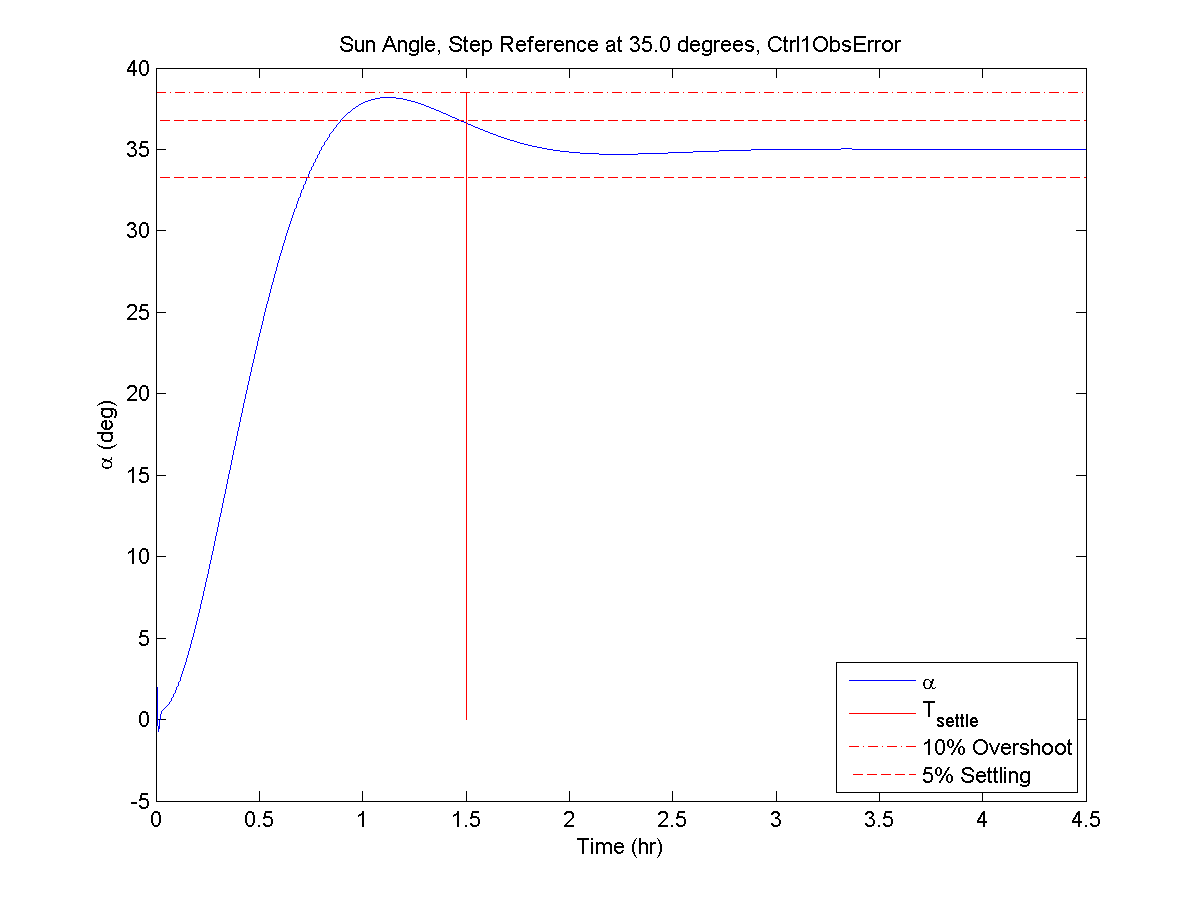
\includegraphics[width = 7.75cm]{Ctrl1ObsError_Alpha.png}
		}
		\subfigure[$\delta$ response]{
			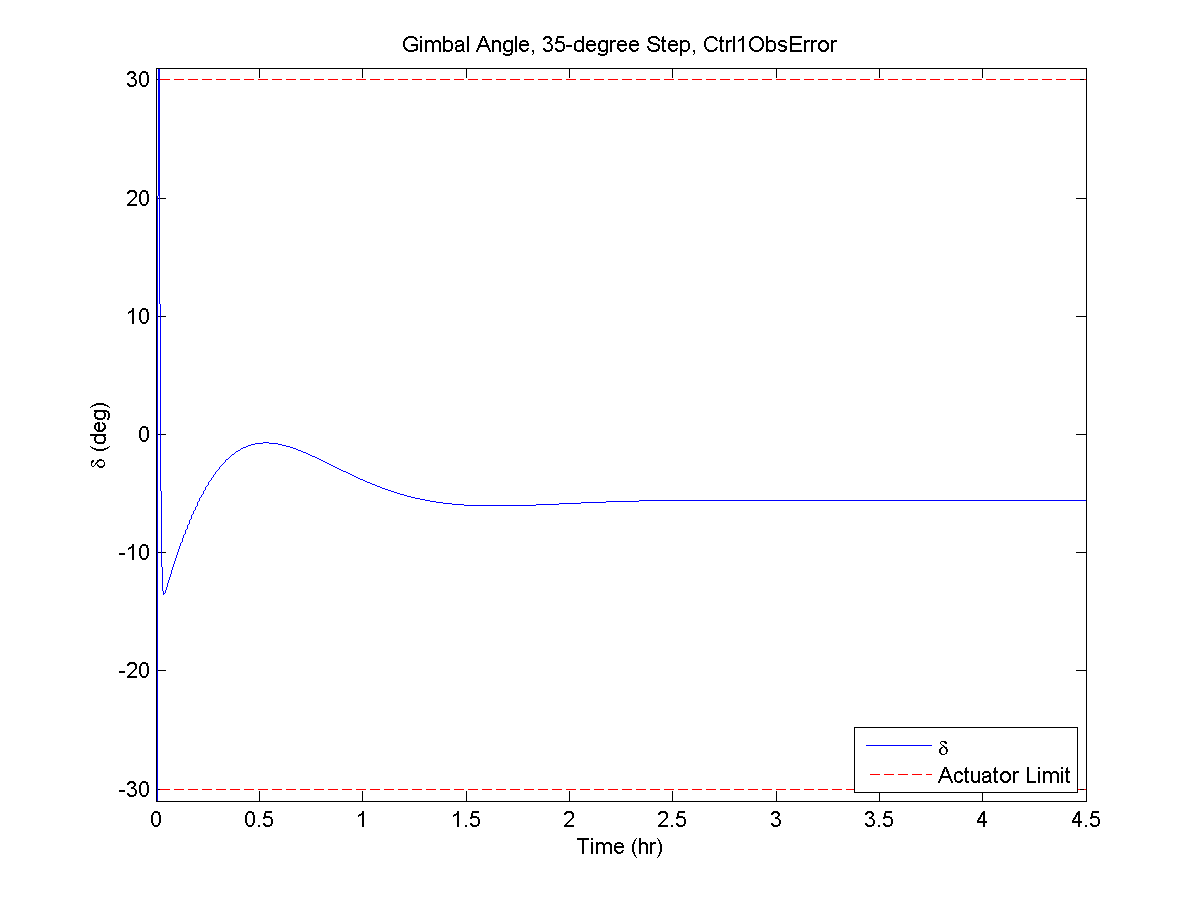
\includegraphics[width = 7.75cm]{Ctrl1ObsError_Delta.png}
		}
		\subfigure[Gimbal torque]{
			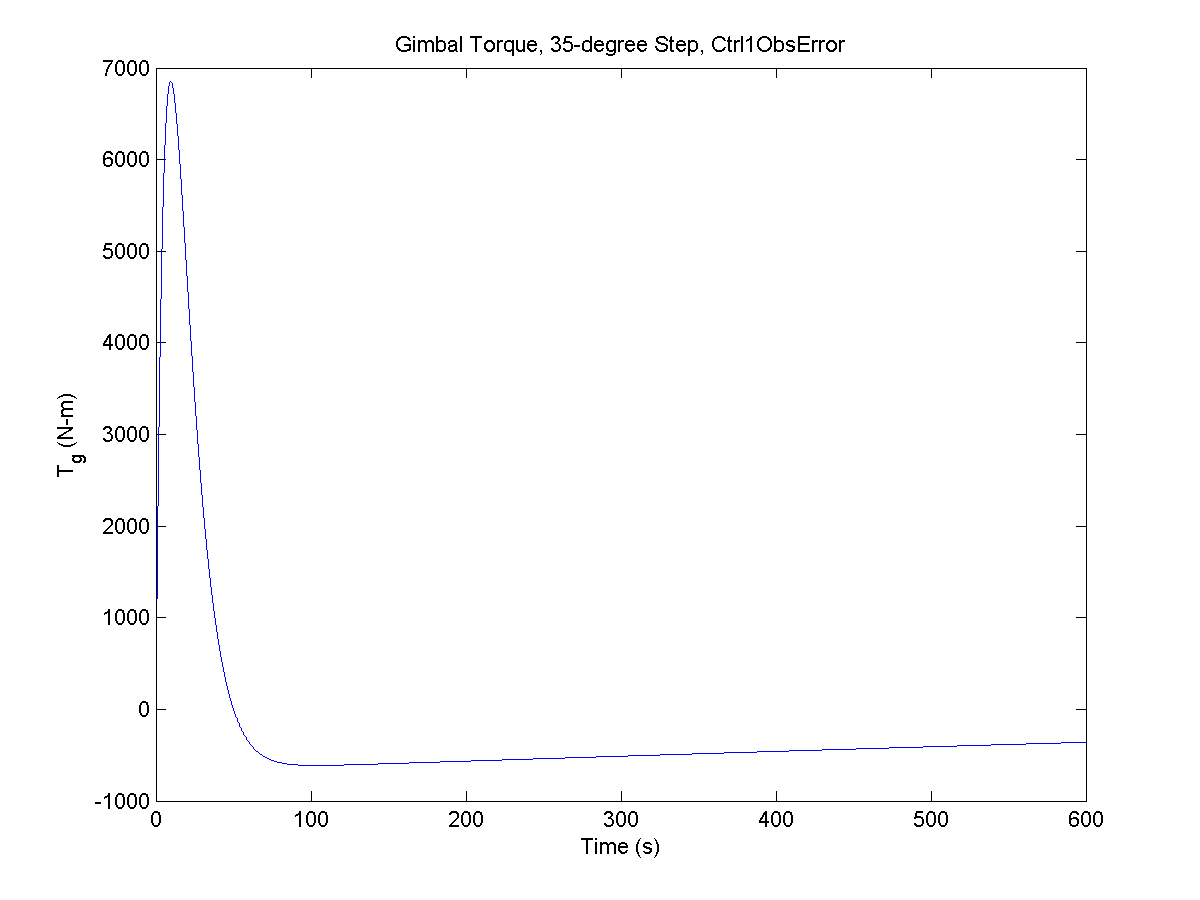
\includegraphics[width = 7.75cm]{Ctrl1ObsError_Torque.png}
		}
		\caption{System response of controller with observer implemented, commanded $\alpha=35^{\circ}$, 0.05$^{\circ}$ sun angle initial error. }
		\label{fig:Controller1Obs}
	\end{figure}	

	The controller still meets the design criteria. However, the torque magnitude is drastically increased, though still feasible to implement on a spacecraft. The additional control effort, which greatly fluctuates the gimbal angle initially, is the most visible result compared to the implementation without the observer. Sensor noise could have a large effect, as the system works hard to rectify a small observer error. Further study should involve realistic sensor noise and filtering techniqes. Figure \ref{fig:Controller1ObsErrors} shows all observer error being driven to zero.

	\begin{figure}[H]
		\centering
		\subfigure[No initial error]{
			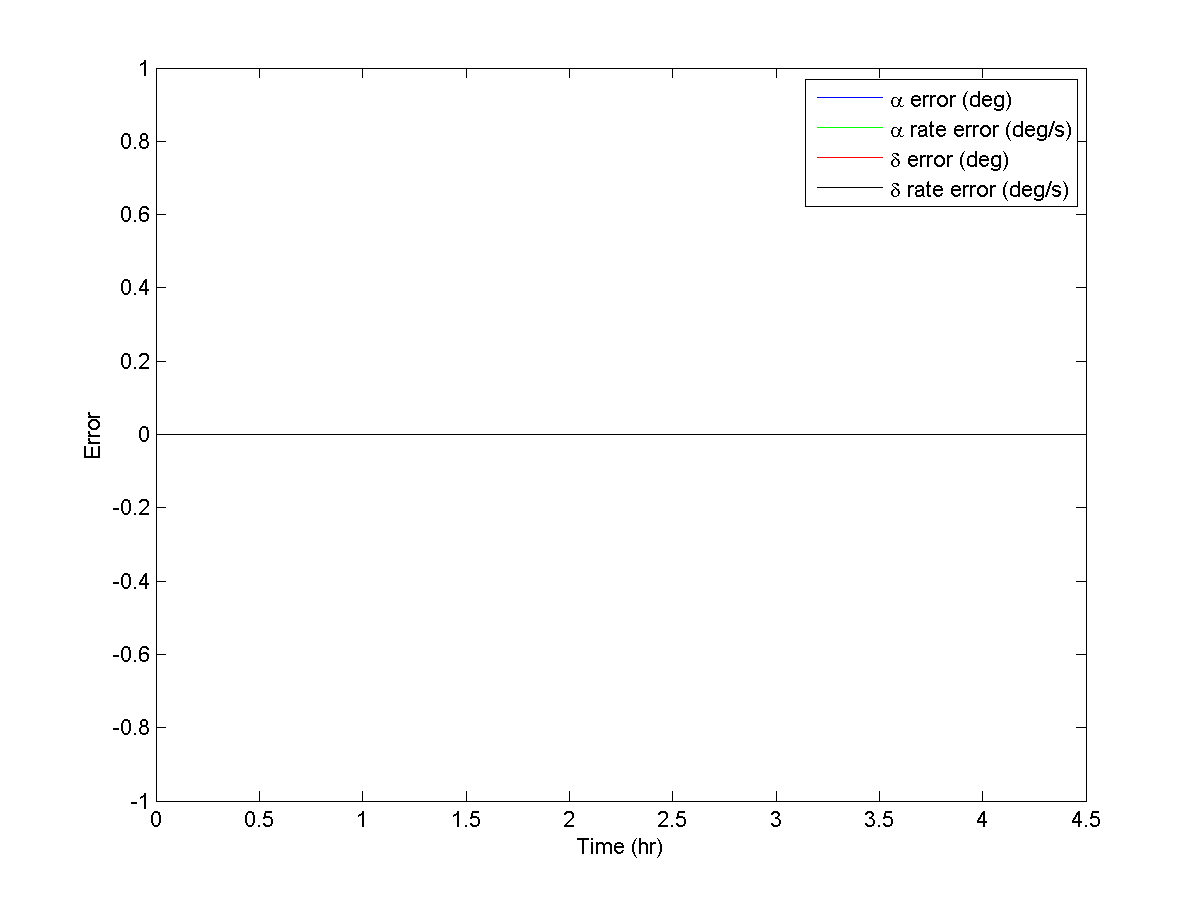
\includegraphics[width = 7.75cm]{Ctrl1Obs_ObsErr.png}
		}
		\subfigure[0.05$^{\circ}$ initial error in sun angle]{
			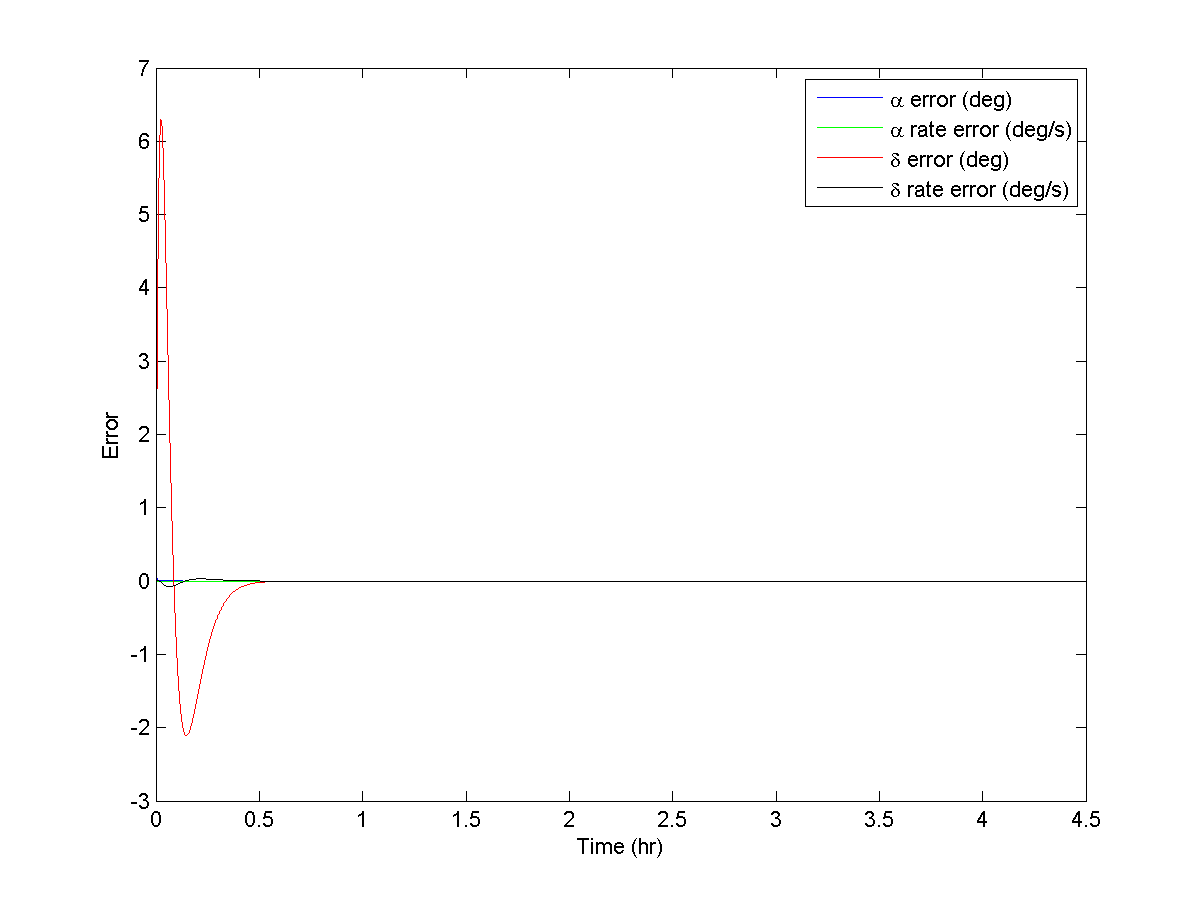
\includegraphics[width = 7.75cm]{Ctrl1ObsError_ObsErr.png}
		}
		\caption{Observer errors. }
		\label{fig:Controller1ObsErrors}
	\end{figure}	

	\section{Optimal Control}

	A linear-quadratic regulator (LQR) controller was implemented, with the cost function
\begin{equation}
J=\int_{0}^{\infty}\left ( x^T(t)Qx(t)+u^T(t)Ru(t) \right )dt
\end{equation}

\noindent
where $Q$ weights the state and $R$ weights the control effort. After tuning with Bryson's method, the weights and resulting gains were found to be
\begin{equation}
\begin{matrix}
Q=diag(\begin{bmatrix}
4.0496\times10^{-9} & 9.9920\times10^{-5} & 3.6446 & 9.9920\times10^{-5} & 9.9920\times10^{-5}
\end{bmatrix})\\ 
R = 10\\ 

K_{LQR}=\begin{bmatrix}
-2.6947 & -1.2308\times10^{-3} & 5.8316\times10^{-1} & -1.4250\times10^{1} & 3.1610\times10^{-3}\end{bmatrix}
\end{matrix}
\end{equation}

Figure \ref{fig:ControllerLQRNom} shows the implementation of the LQR controller with the previously-derived observer, without initial observer error.

	\begin{figure}[H]
		\centering
		\subfigure[$\alpha$ response]{
			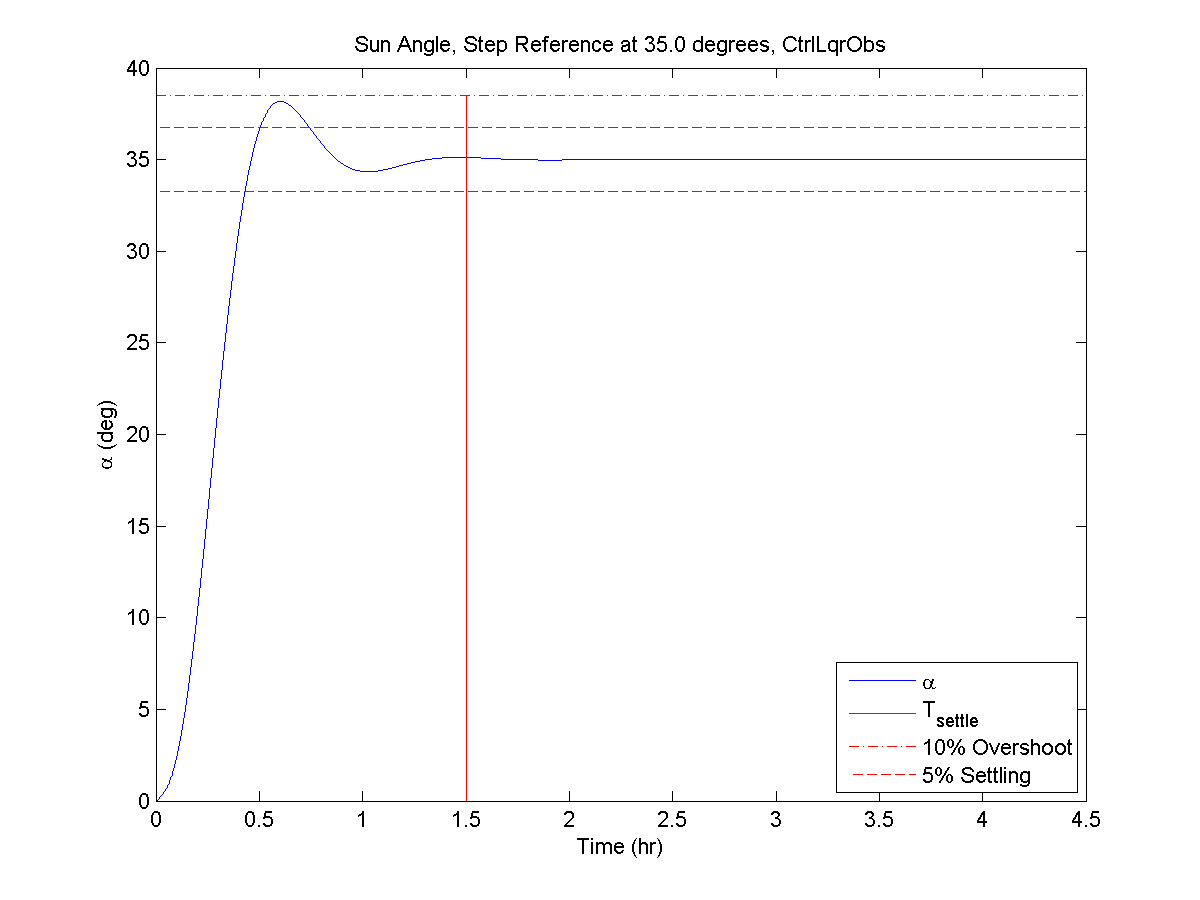
\includegraphics[width = 7.75cm]{CtrlLqrObs_Alpha.png}
		}
		\subfigure[$\delta$ response]{
			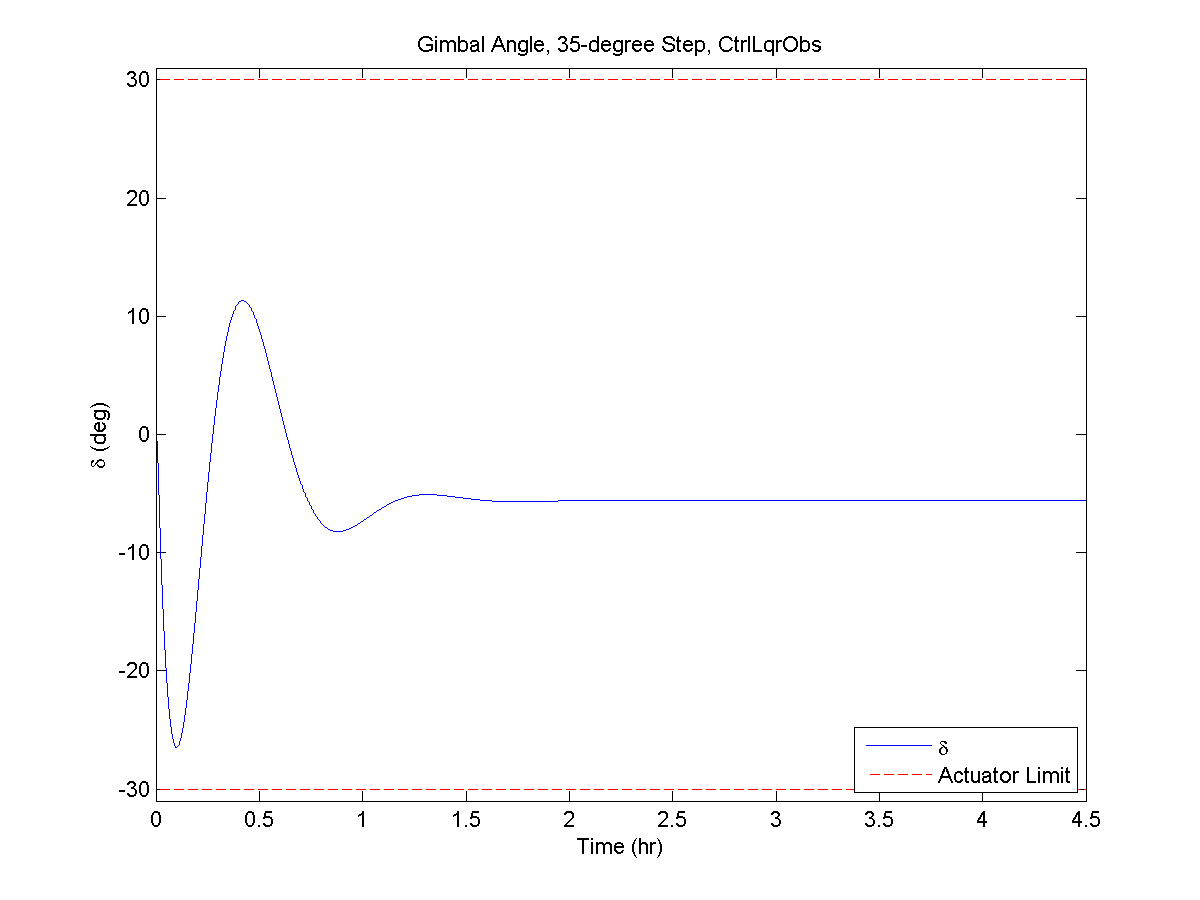
\includegraphics[width = 7.75cm]{CtrlLqrObs_Delta.png}
		}
		\subfigure[Gimbal torque]{
			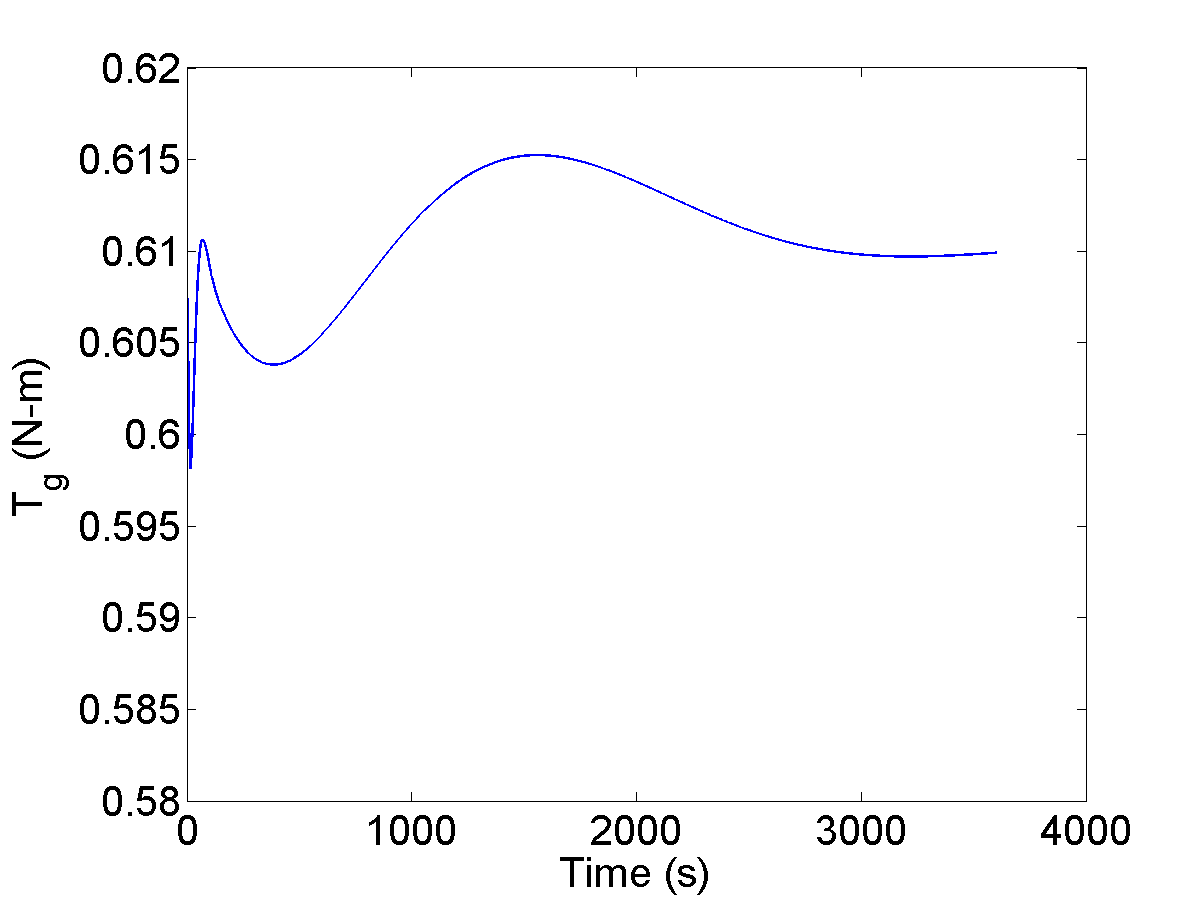
\includegraphics[width = 7.75cm]{CtrlLqrObs_Torque.png}
		}
		\caption{System response of LQR controller with observer implemented, commanded $\alpha=35^{\circ}$ }
		\label{fig:ControllerLQRNom}
	\end{figure}	

	The LQR controller settles considerably better than the one with manually-placed poles using a SISO technique. The gimbal angle fluctuates more, but again settles to its trim state for the commanded $\alpha$. The control effort is only slightly less than the first controller, but the LQR control effort fluctuates more (note the differing time scales on the torque plots).

	\vspace{5 mm}

	The response of the LQR controller implemented with observer error can be seen in Figure \ref{fig:ControllerLQRErr}.

	\begin{figure}[H]
		\centering
		\subfigure[$\alpha$ response]{
			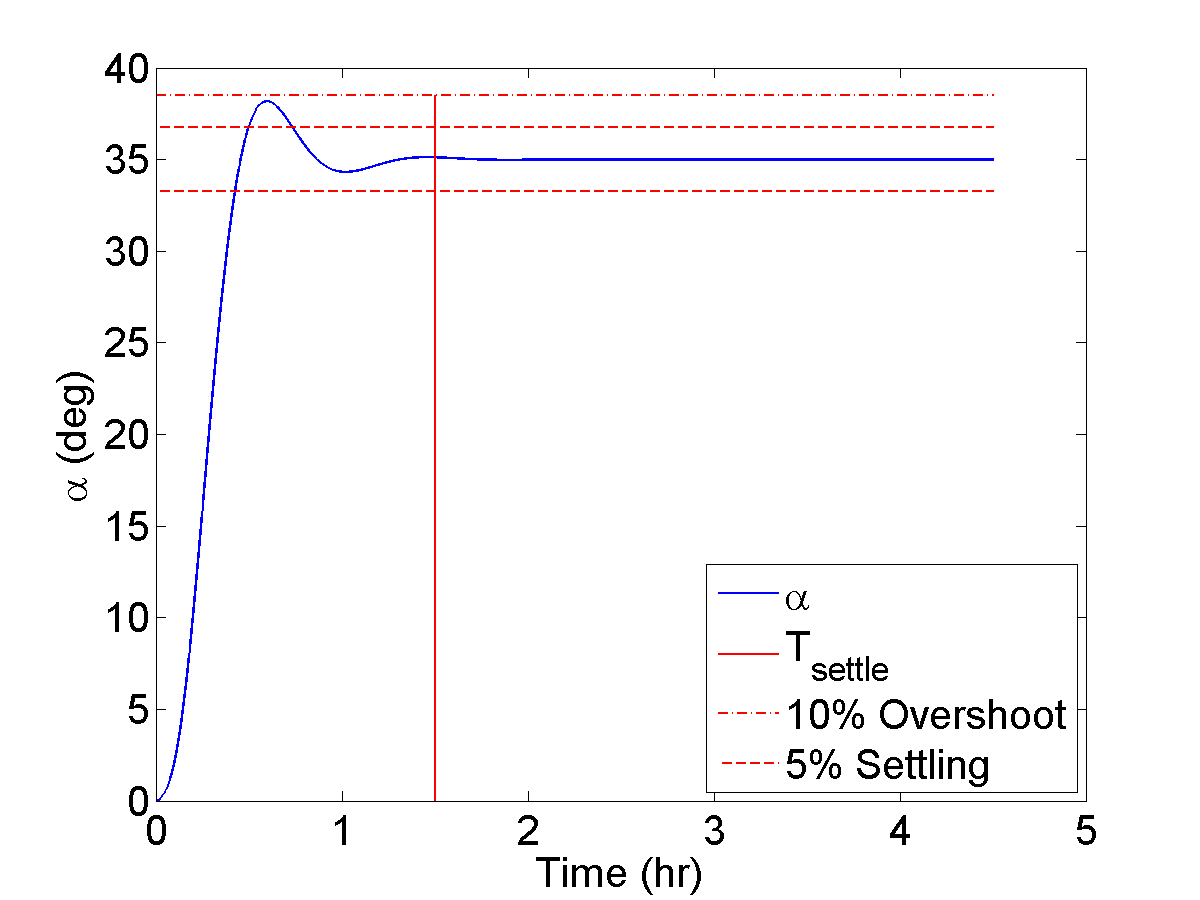
\includegraphics[width = 7.75cm]{CtrlLqrObsError_Alpha.png}
		}
		\subfigure[$\delta$ response]{
			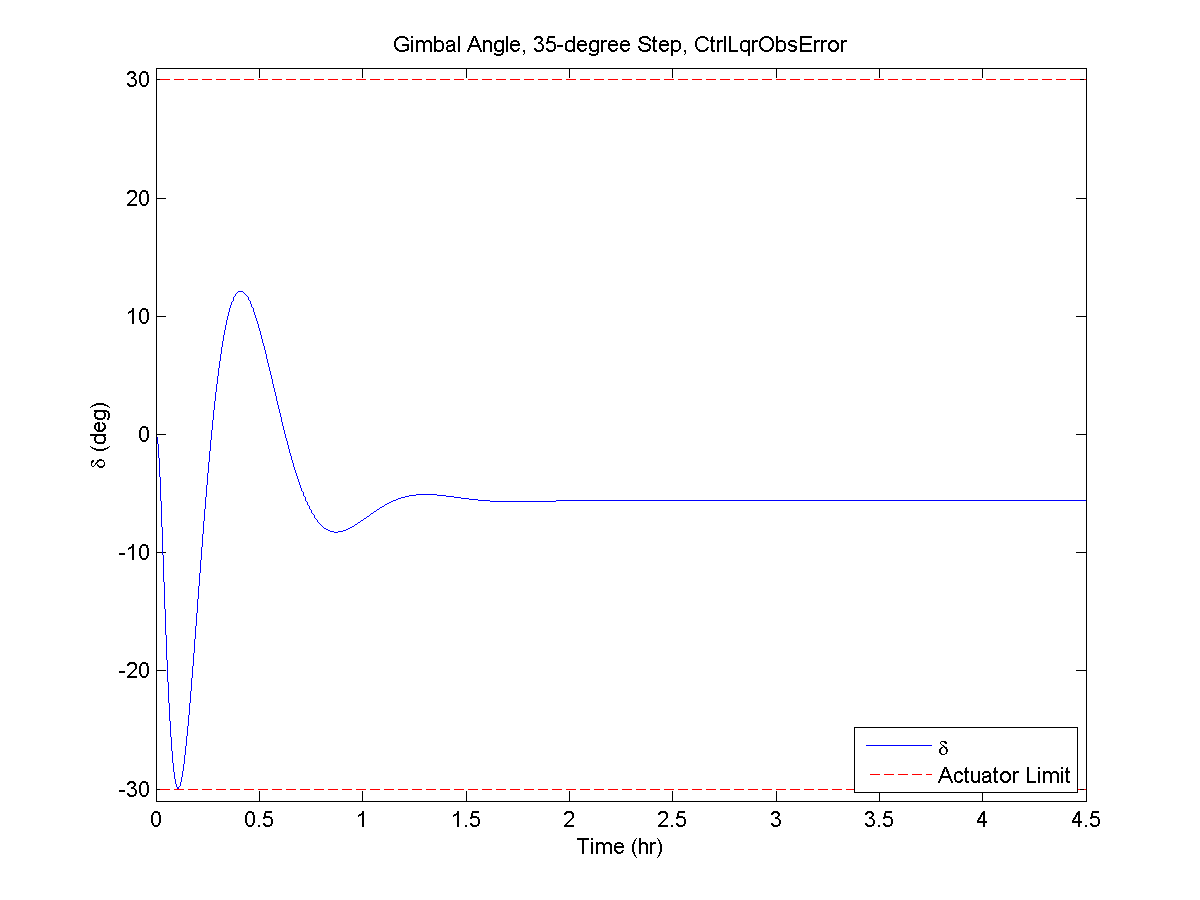
\includegraphics[width = 7.75cm]{CtrlLqrObsError_Delta.png}
		}
		\subfigure[Gimbal torque]{
			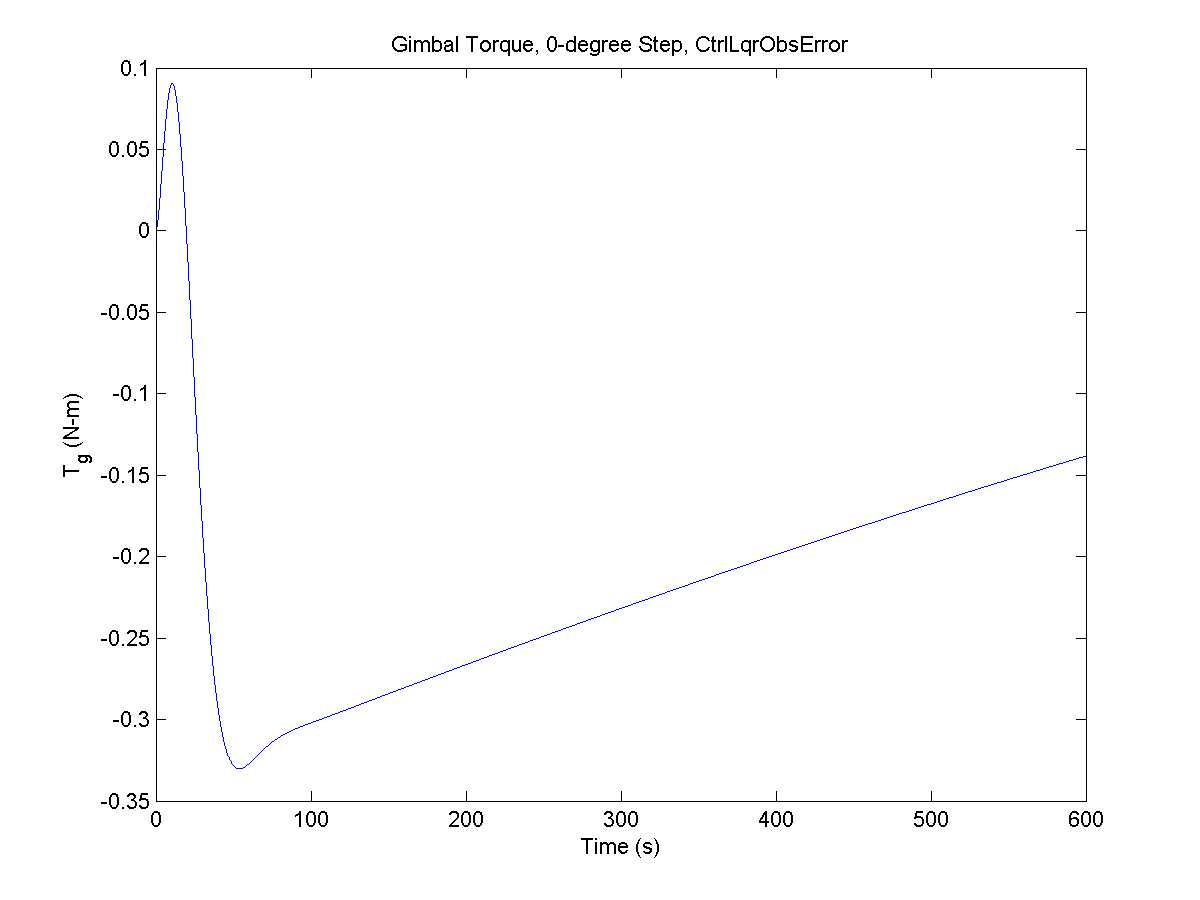
\includegraphics[width = 7.75cm]{CtrlLqrObsError_Torque.png}
		}
		\caption{System response of LQR controller with observer implemented, commanded $\alpha=35^{\circ}$, initial observer error }
		\label{fig:ControllerLQRErr}
	\end{figure}	

	Despite observer error, the LQR controller still settles quickly. Gimbal angle comes very close to the limit, but is still within the boundary. The control torque is considerably less than the first controller's with the same observer error. The lesser control effort makes this response more desirable than the first controller's response. Observer error can be seen in Figure \ref{fig:ControllerLQRObsErrors}.

	\begin{figure}[H]
		\centering
		\subfigure[No initial error]{
			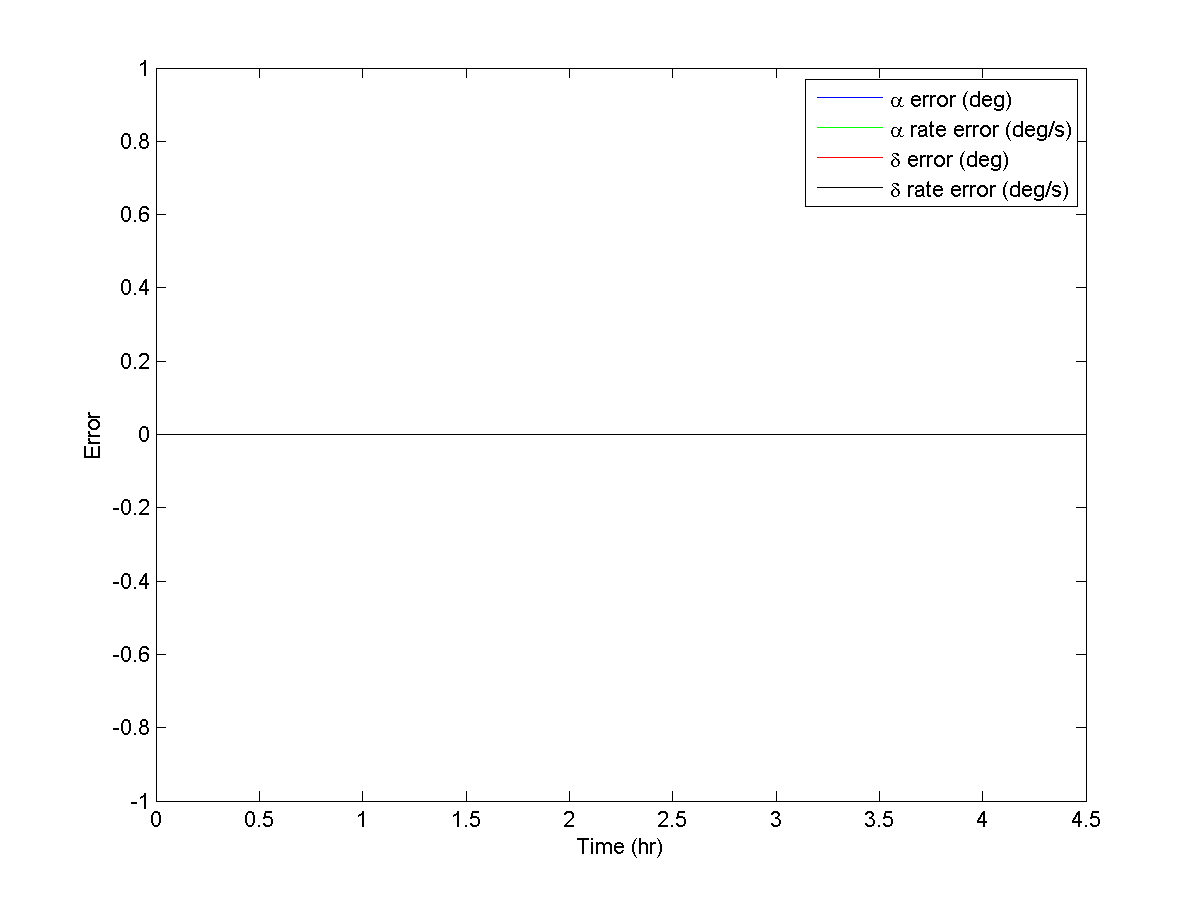
\includegraphics[width = 7.75cm]{CtrlLqrObs_ObsErr.png}
		}
		\subfigure[0.05$^{\circ}$ initial error in sun angle]{
			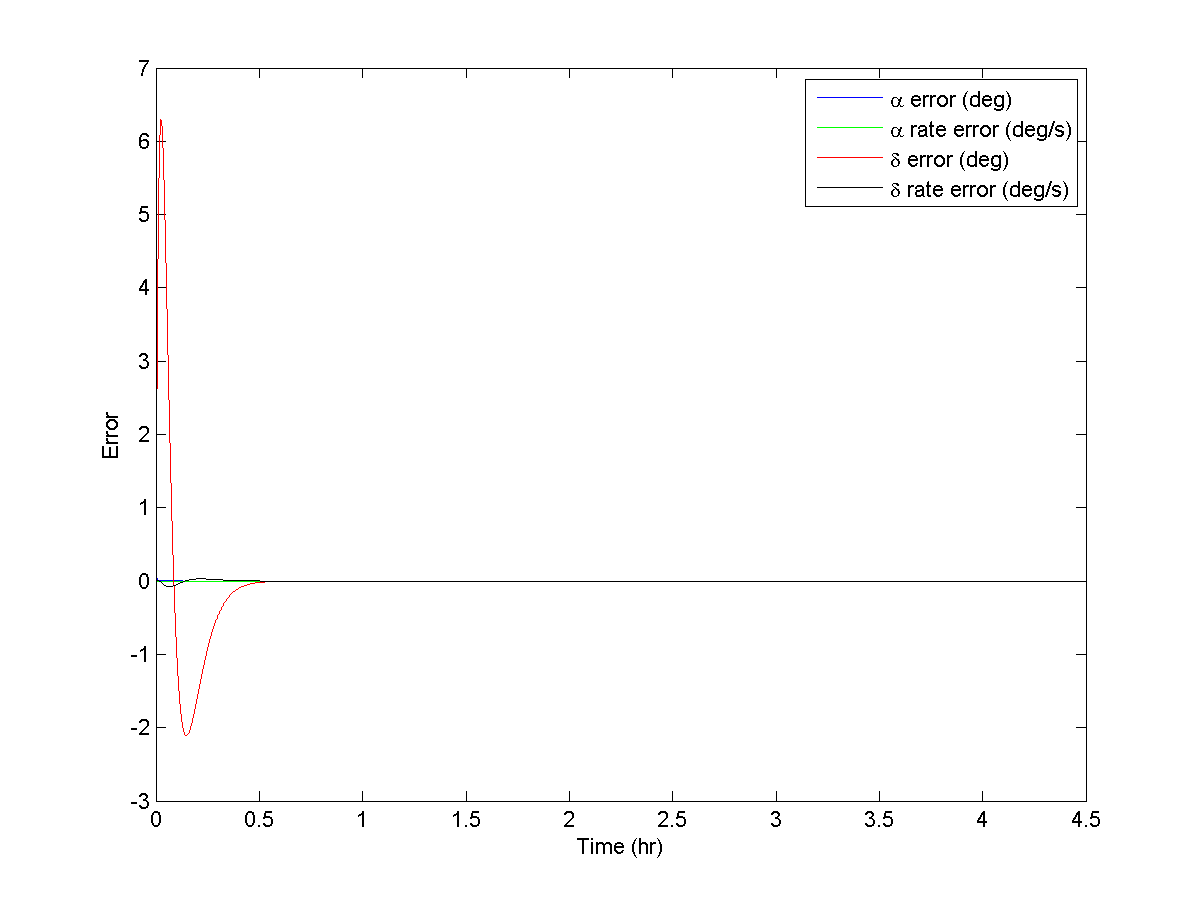
\includegraphics[width = 7.75cm]{CtrlLqrObsError_ObsErr.png}
		}
		\caption{Observer errors. }
		\label{fig:ControllerLQRObsErrors}
	\end{figure}	

	The observer error goes to zero in the same way the first controller-observer implementation did. Due to the difference being imperceivable, the difference in error is provided in Figure \ref{fig:DiffInError}.

	\begin{figure}[H]
		\centering
			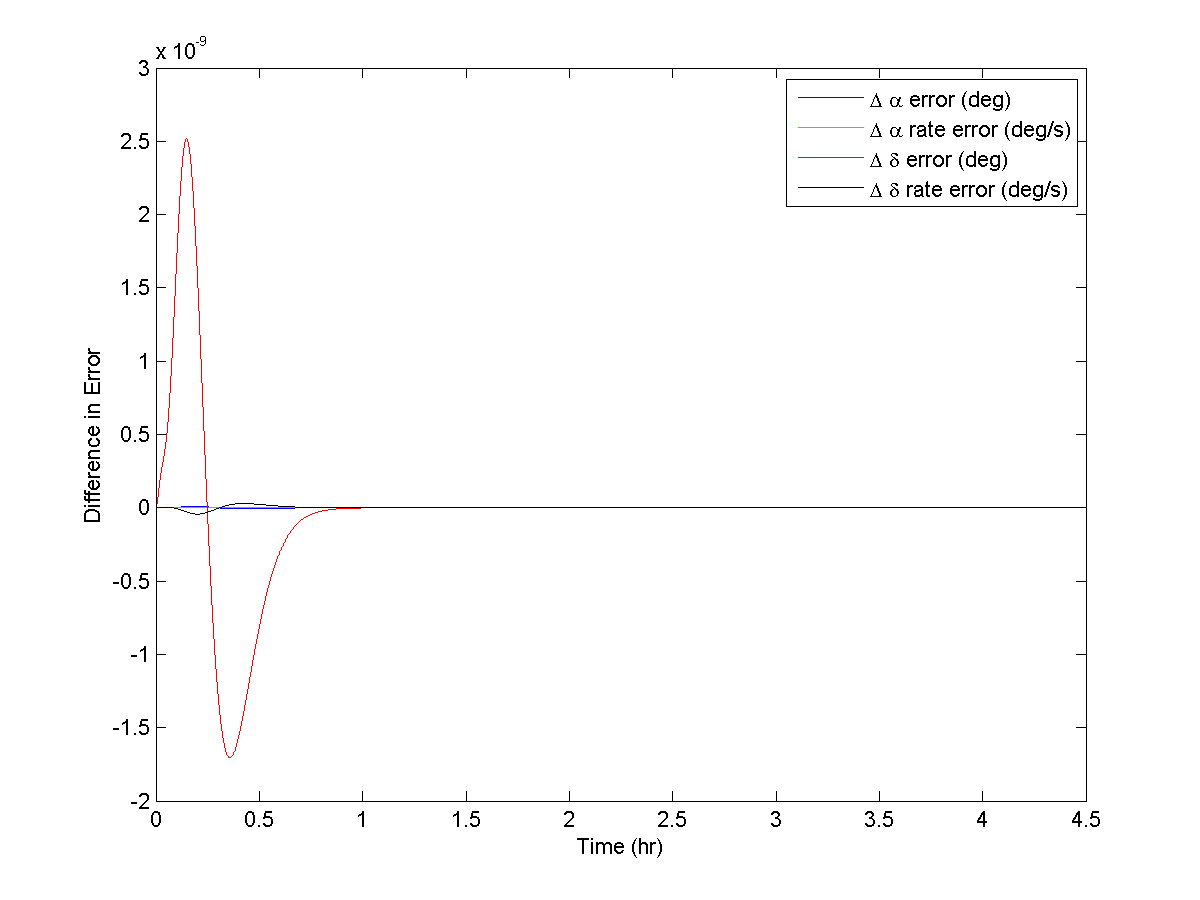
\includegraphics[width = 7.75cm]{Ctrl1_LQR_error_diff_ObsErr.png}
		\caption{Observer errors with LQR control. }
		\label{fig:DiffInError}
	\end{figure}	

%    \section{Appendix B}
%This appendix contains all Matlab code used by the authors to analyize their data.
%    
%    \lstset{language=Matlab,%
%    	%basicstyle=\color{red},
%    	breaklines=true,%
%    	morekeywords={matlab2tikz},
%    	keywordstyle=\color{blue},%
%    	morekeywords=[2]{1}, keywordstyle=[2]{\color{black}},
%    	identifierstyle=\color{black},%
%    	stringstyle=\color{mylilas},
%    	commentstyle=\color{mygreen},%
%    	showstringspaces=false,%without this there will be a symbol in the places where there is a space
%    	numbers=left,%
%    	numberstyle={\tiny \color{black}},% size of the numbers
%    	numbersep=9pt, % this defines how far the numbers are from the text
%    	emph=[1]{for,end,break},emphstyle=[1]\color{red}, %some words to emphasise
%    	%emph=[2]{word1,word2}, emphstyle=[2]{style},   
%    }
    
%    \lstinputlisting{ASEN5090_ecef2azelrange.m}
%    \vspace{5mm}
%    
%    \lstinputlisting{ASEN5090_GPSvis.m}
%    \vspace{5mm}
%\lstinputlisting{HW5_rel_err.m}
%\vspace{5mm}
%\lstinputlisting{import_gps_data.m}
%\vspace{5mm}
%\lstinputlisting{datenum8601.m}
%\vspace{5mm}
%\lstinputlisting{lab_err_plots.m}
%\vspace{5mm}
	
\end{document}

% - Release $Name:  $ -
